\documentclass[12pt,a4paper]{article}
\usepackage[utf8]{inputenc}
\usepackage[french]{babel}
\usepackage[T1]{fontenc}
\usepackage{graphicx}
\usepackage{xcolor}
\usepackage[left=2cm,right=2cm,top=2cm,bottom=2cm]{geometry}
\begin{document}

\section*{\begin{center}
Mes notes
\end{center}}

\begin{center}
	\textbf{que veut dire calibrage/étalonnage? }
\end{center}
\textbf{calibrage/étalonnage de la caméras}: c'est le réglage des fonctionnalité de la caméras pour arriver à faire ce qu'on veut
\\
\begin{center}
\textbf{quel est l'objectif du sujet?}
\end{center}
 c'est de pouvoir prendre une photo et mesurer la longueur du saut en longueur par rapport à la ligne de départ avec la caméras.\\
 \\
 \textbf{première position :}\\
il faut d'abord arriver à mesurer en plaçant le bois c'est à dire placer le bois là où la personne est tombé et ensuite prendre
une image à partir du point de départ jusqu'au niveau du bois et ensuite calculer la distance à partir de la photo.\\
\\
\textbf{deuxième position :}
Par la suite arriver à programmer la caméras de telle sorte qu'elle puisse prendre les photos automatiquement à la détection de la personne(prendre une photos au départ , au milieu et à l'atterrissage),  utiliser un capteur de son aussi et calculer la distance à partir de ces photos sans l'intervention d'une personne. 
\\
 \begin{center}
 	\textbf{Comment arriver à faire cela?}\\
 \end{center}

 

\textbf{première position :} apprendre l'IA à maitriser les images et reconnaitre les différents objets en rapport avec les sauts.
\begin{itemize}
\item l'apprendre à connaitre le sable, la ligne d'appel,les bordures de la zone de réception, le bois pour représenté le point d' atterrissage 
\item une fois le premier item atteint , l'apprendre à détecter les images des humains, à reconnaitre lorsque l'athlète a mordu ou est dans les normes, considérer la marque la plus proche de la ligne d'appel comme point d'atterrissage,voir si l'athlète a fait une faute de sortie ou non en détectant sa sortie par rapport au point d'atterrissage. \\
\end{itemize}

\textbf{deuxième position :} écrire un algorithme qui permet de calculer la distance et l'intégrer dans l'IA \\
\\
\textbf{troisième position :} régler la caméra pour qu'elle puisse prendre la photo, l'envoyer vers un lieu de stockage. Lier l'IA avec la caméras et une fois le calcul finis ,il affiche le résultat sur l'écran.
\\
\begin{center}
\textbf{I.comment créer l'IA?}\\	
\end{center}


\textbf{A.D'après mes recherches du 13/02/2024,je retiens ceci pour débuter:\\}

\begin{itemize}
	\item définir le type d'objet que l'IA doit utiliser(sable,la ligne d'appel,les bordures de la zone de réception, le bois) et dans le contexte que je que je veux l'utiliser (sauts en longueur)
	\item Collecter plusieurs images sur les objets avec une bonne précision
	\item choisir un framework d'apprentissage automatique"open-source" (TensorFlow, PyTorch, Opencv et Halide)
	\item Pour entrainer mon modèle
	Divisez mes données en deux ensembles : un ensemble d'apprentissage et un ensemble de test.
	\begin{itemize}	
		\item Utilisez l'ensemble d'apprentissage pour entraîner mon modèle d'IA à reconnaître les objets dans les images.
		\item Évaluez la performance de mon modèle sur l'ensemble de test et apportez les ajustements nécessaires.\\
   \end{itemize}
\end{itemize}

\begin{center}
	\textbf{B.Recherche du 14/02/2024\\}
\end{center}


Les différents frameworks adaptés à mon projet:\\

1.OpenCV:\\

Bibliothèque open-source largement utilisée pour le traitement d'image et la vision par ordinateur.
Offre des fonctions pour l'acquisition d'images, le prétraitement, l'étalonnage de la caméra, la détection de caractéristiques et la reconstruction 3D.
Large communauté d'utilisateurs et de développeurs, documentation complète et nombreux tutoriels disponibles.\\

2. TensorFlow:\\

TensorFlow est une plateforme open-source développée par Google pour le machine learning et le deep learning, mais elle comprend également des modules pour le traitement d'images.
TensorFlow propose TensorFlow Image Processing (TFLearn), qui fournit des outils pour la préparation, la manipulation et le traitement d'images dans le contexte de l'apprentissage automatique.\\

3.PyTorch\\

PyTorch est un autre framework open-source développé principalement par Facebook AI Research (FAIR) pour le deep learning.
Bien qu'il soit principalement utilisé pour le deep learning, PyTorch offre également des fonctionnalités de traitement d'image, notamment pour la manipulation d'images et le prétraitement des données.\\

4. Halide:\\

Langage de programmation pour le traitement d'image et la génération de code optimisé pour différents types de processeurs.
Permet de créer des pipelines de traitement d'image performants et flexibles.
Nécessite des connaissances en programmation et en parallélisation.\\

\textbf{Pourquoi ce choix?\\}

J'ai décidé d'utiliser OpenCV car il est open-source, il offre une multitude de fonctionnalités pour le traitement d'image, y compris la calibration de caméra, la détection d'objets, le suivi de mouvement et la segmentation d'image.il a une très grande documentation , il a une communauté active , il est compatible avec plusieurs langage de programmation(python,c++,java), il est utilisable sur plusieurs plateforme.
Avec toutes ces paramètres il est le mieux adapté à mon projet.\\

\textbf{Python} sera le langage que je vais utiliser car  il est le seul que je ne connais pas.\\

\begin{center}
	\textbf{C.Recherche du 15/02/2024\\}
\end{center}


\textbf{je débute avec OpenCv avec Python par le tutoriel du site officiel OpenCv \cite{noauthor_opencv_2020}}

\begin{center}
	\textbf{1.Vue d'ensemble}
\end{center}
\begin{itemize}
	\item \textbf{La vision par ordinateur} est un processus par lequel nous pouvons comprendre les images et les vidéos , comment elle sont stocker et comment nous pouvons les manipuler et en extraire des données.\\
	 
	\item \textbf{Le traitement d'image} est une méthode permettant d'effectuer certaines opérations sur une image numérique,afin d'obtenir une image améliorée et/ou d'en extraire des informations utiles.  \\
	Elle comprends essentiellement trois étapes:\\
	a.Importation de l’image\\
	b.Analyser et manipuler l’image\\
	c.Sortie dans laquelle le résultat peut être modifié : image ou rapport basé sur l’analyse d’image\\
	
	\item \textbf{Une image} est une matrice bidimensionnelle(3D dans le cas d'images colorées)
	qui est défini par la fonction mathématique	 f(x, y) à tout point donne la valeur du pixel à ce point d’une image, la valeur du pixel décrit la luminosité de ce pixel et sa couleur.\\
	
	\item \textbf{Comment l'ordinateur lit'il l'image?\\}
	
	L'ordinateur lit n'importe quelle image sous la forme d'une plage de valeurs comprise entre 0 et 255.C'est à dire que dans une image numérique, chaque pixel est associé à une valeur qui représente son intensité lumineuse ou sa couleur. Ces valeurs sont généralement représentées en niveaux de gris(compris entre 0et255) pour les images en noir(représenté par 0) et blanc(représenté par 255), ou en combinaisons de couleurs(rouge,vert et bleue) pour les images en couleur.Chaque composante(rouge,vert et bleue) représentée par une valeur comprise entre 0 et 255, où 0 représente l'absence de cette couleur et 255 représente une saturation maximale de cette couleur.\\	
\end{itemize}

\begin{center}
	\textbf{2.Installation d'OpenCv sur linux}\textcolor{red}{À ajouter dans le calibrage, la partie installation des dépendances}
\end{center}

Pour installer OpenCV, il faut avoir Python et PIP, préinstallés sur mon système. 

\begin{center}
	\textbf{2.a Vérification}
\end{center}

Vérifions pour voir si Python et pip sont installés
\begin{itemize}
\item \textbf{Ouvrir le terminal en tapant Ctrl+Alt+T }
\item \textbf{Taper python - -version ou python3.10 - -version } pour vérifier pour python\\
Si il est déjà installé, il générera un message avec la version Python disponible. Dans notre cas il est déjà installé car la plupart des systèmes d'exploitations Linux ont Python préinstallé. Si il n'est pas installé on peut l'installer en suivant les instructions de ce site.\cite{noauthor_comment_nodate} \\
Python est un langage de programmation généraliste de haut niveau largement utilisé. Il permet de travailler rapidement et d'intégrer des systèmes plus efficacement. Il existe deux versions principales de Python : Python 2 et Python 3 . Les deux sont assez différents. Nous avons la dernière version qui est 3.10.12\\

\item \textbf{Taper pip3 - -version} pour voir si pip est installé ; dans notre cas il n'est pas installé \\
\end{itemize}

\includegraphics[scale=0.7]{image/Verification(python et pip).png}


\begin{center}
	\textbf{2.b Installation de pip3 \cite{noauthor_comment_nodate-1}}
\end{center}

PIP est un système de gestion de packages utilisé pour installer et gérer des packages logiciels/bibliothèques écrits en Python. Ces fichiers sont stockés dans un grand « référentiel en ligne » appelé Python Package Index (PyPI).PIP est le programme d'installation du package pour Python 2 et pip3 est spécialement conçu pour Python 3. Le nom « pip » est un acronyme récursif qui signifie « Pip Installs Packages » ou « Pip Installs Python ». \\
\begin{itemize}
\item \textbf{Taper sudo apt update} pour mettre à jour tout les paquets installé
\item \textbf{Taper sudo apt-get install python3-pip} \\
\end{itemize}
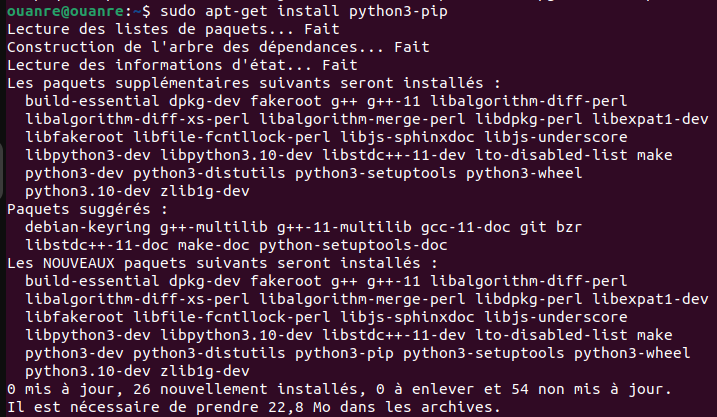
\includegraphics[scale=0.5]{image/instalation de pip3.png} \\

\includegraphics[scale=0.5]{image/pip3 installé.png}

\begin{center}
	\textbf{2.c Téléchargement et Installation de Opencv}
\end{center}
OpenCV peut être directement téléchargé et installé à l'aide de pip (gestionnaire de packages). \\
\begin{itemize}
\item \textbf{Taper sudo apt update}
\item \textbf{Taper sudo apt install python-opencv} pour l'installation d'opencv \\

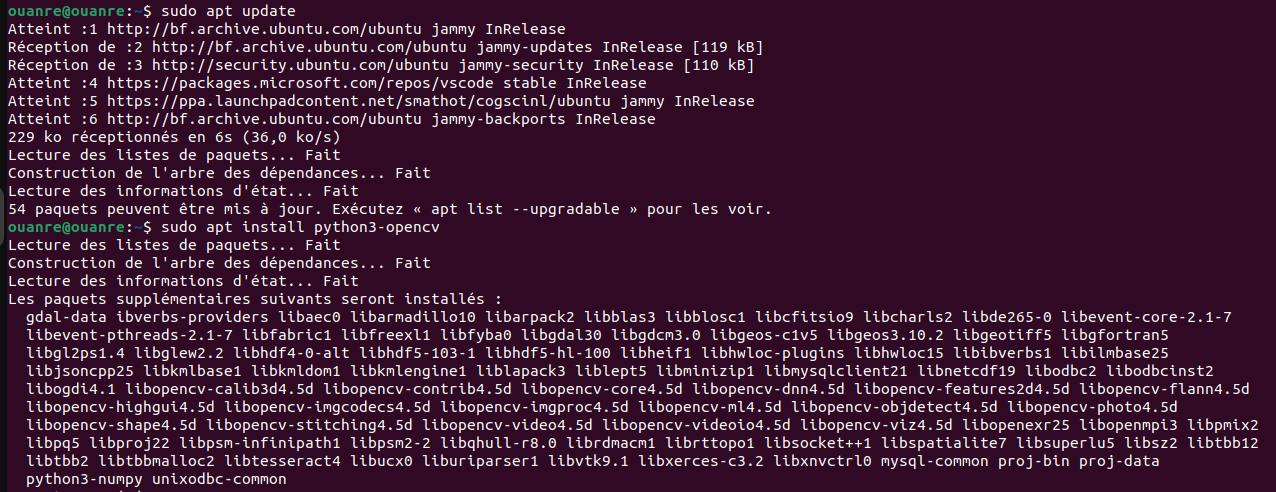
\includegraphics[scale=0.36]{image/insallation opencv.png}\\

\item \textbf{Taper python3} pour vérifier de la version que nous venons d'installer \\

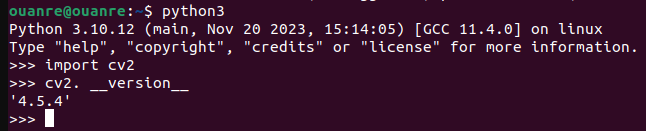
\includegraphics[scale=0.5]{image/verification opencv.png}\\

\item \textbf{Taper sudo apt update}
\item \textbf{Taper pip3 install opencv-python} pour l'installation des packages d'open cv\\

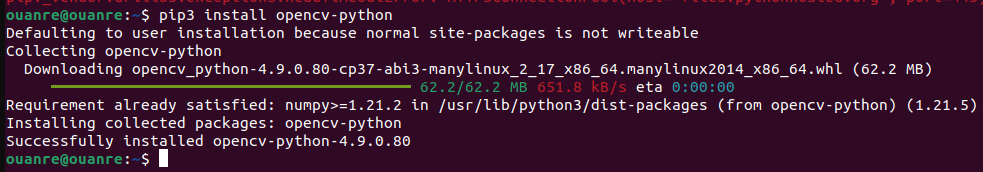
\includegraphics[scale=0.5]{image/package opencv.png}\\
 
 Lors de l'installation des packages opencv sera mis à jour automatiquement donc il quitte de la version 4.5.4 à 4.9.0
 
\item \textbf{Taper python3} pour vérifier de la version que nous venons d'installer \\

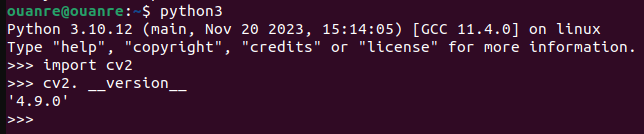
\includegraphics[scale=0.5]{image/verification package opencv.png}\\

\end{itemize}











































\newpage
\bibliographystyle{smfplain}
	\bibliography{mybiblio}
\end{document}